\documentclass[english, 11 pt, class=article, crop=false]{standalone}
\usepackage[T1]{fontenc}
%\renewcommand*\familydefault{\sfdefault} % For dyslexia-friendly text
\usepackage{lmodern} % load a font with all the characters
\usepackage{geometry}
\geometry{verbose,paperwidth=16.1 cm, paperheight=24 cm, inner=2.3cm, outer=1.8 cm, bmargin=2cm, tmargin=1.8cm}
\setlength{\parindent}{0bp}
\usepackage{import}
\usepackage[subpreambles=false]{standalone}
\usepackage{amsmath}
\usepackage{amssymb}
\usepackage{esint}
\usepackage{babel}
\usepackage{tabu}
\makeatother
\makeatletter

\usepackage{titlesec}
\usepackage{ragged2e}
\RaggedRight
\raggedbottom
\frenchspacing

% Norwegian names of figures, chapters, parts and content
\addto\captionsenglish{\renewcommand{\figurename}{Figur}}
\makeatletter
\addto\captionsenglish{\renewcommand{\chaptername}{Kapittel}}
\addto\captionsenglish{\renewcommand{\partname}{Del}}


\usepackage{graphicx}
\usepackage{float}
\usepackage{subfig}
\usepackage{placeins}
\usepackage{cancel}
\usepackage{framed}
\usepackage{wrapfig}
\usepackage[subfigure]{tocloft}
\usepackage[font=footnotesize,labelfont=sl]{caption} % Figure caption
\usepackage{bm}
\usepackage[dvipsnames, table]{xcolor}
\definecolor{shadecolor}{rgb}{0.105469, 0.613281, 1}
\colorlet{shadecolor}{Emerald!15} 
\usepackage{icomma}
\makeatother
\usepackage[many]{tcolorbox}
\usepackage{multicol}
\usepackage{stackengine}

\usepackage{esvect} %For vectors with capital letters

% For tabular
\usepackage{array}
\usepackage{multirow}
\usepackage{longtable} %breakable table

% Ligningsreferanser
\usepackage{mathtools}
\mathtoolsset{showonlyrefs}

% index
\usepackage{imakeidx}
\makeindex[title=Indeks]

%Footnote:
\usepackage[bottom, hang, flushmargin]{footmisc}
\usepackage{perpage} 
\MakePerPage{footnote}
\addtolength{\footnotesep}{2mm}
\renewcommand{\thefootnote}{\arabic{footnote}}
\renewcommand\footnoterule{\rule{\linewidth}{0.4pt}}
\renewcommand{\thempfootnote}{\arabic{mpfootnote}}

%colors
\definecolor{c1}{cmyk}{0,0.5,1,0}
\definecolor{c2}{cmyk}{1,0.25,1,0}
\definecolor{n3}{cmyk}{1,0.,1,0}
\definecolor{neg}{cmyk}{1,0.,0.,0}

% Lister med bokstavar
\usepackage[inline]{enumitem}

\newcounter{rg}
\numberwithin{rg}{chapter}
\newcommand{\reg}[2][]{\begin{tcolorbox}[boxrule=0.3 mm,arc=0mm,colback=blue!3] {\refstepcounter{rg}\phantomsection \large \textbf{\therg \;#1} \vspace{5 pt}}\newline #2  \end{tcolorbox}\vspace{-5pt}}

\newcommand\alg[1]{\begin{align} #1 \end{align}}

\newcommand\eks[2][]{\begin{tcolorbox}[boxrule=0.3 mm,arc=0mm,enhanced jigsaw,breakable,colback=green!3] {\large \textbf{Eksempel #1} \vspace{5 pt}\\} #2 \end{tcolorbox}\vspace{-5pt} }

\newcommand{\st}[1]{\begin{tcolorbox}[boxrule=0.0 mm,arc=0mm,enhanced jigsaw,breakable,colback=yellow!12]{ #1} \end{tcolorbox}}

\newcommand{\spr}[1]{\begin{tcolorbox}[boxrule=0.3 mm,arc=0mm,enhanced jigsaw,breakable,colback=yellow!7] {\large \textbf{Språkboksen} \vspace{5 pt}\\} #1 \end{tcolorbox}\vspace{-5pt} }

\newcommand{\sym}[1]{\colorbox{blue!15}{#1}}

\newcommand{\info}[2]{\begin{tcolorbox}[boxrule=0.3 mm,arc=0mm,enhanced jigsaw,breakable,colback=cyan!6] {\large \textbf{#1} \vspace{5 pt}\\} #2 \end{tcolorbox}\vspace{-5pt} }

\newcommand\algv[1]{\vspace{-11 pt}\begin{align*} #1 \end{align*}}

\newcommand{\regv}{\vspace{5pt}}
\newcommand{\mer}{\textsl{Merk}: }
\newcommand{\mers}[1]{{\footnotesize \mer #1}}
\newcommand\vsk{\vspace{11pt}}
\newcommand\vs{\vspace{-11pt}}
\newcommand\vsb{\vspace{-16pt}}
\newcommand\sv{\vsk \textbf{Svar} \vspace{4 pt}\\}
\newcommand\br{\\[5 pt]}
\newcommand{\figp}[1]{../fig/#1}
\newcommand\algvv[1]{\vs\vs\begin{align*} #1 \end{align*}}
\newcommand{\y}[1]{$ {#1} $}
\newcommand{\os}{\\[5 pt]}
\newcommand{\prbxl}[2]{
\parbox[l][][l]{#1\linewidth}{#2
	}}
\newcommand{\prbxr}[2]{\parbox[r][][l]{#1\linewidth}{
		\setlength{\abovedisplayskip}{5pt}
		\setlength{\belowdisplayskip}{5pt}	
		\setlength{\abovedisplayshortskip}{0pt}
		\setlength{\belowdisplayshortskip}{0pt} 
		\begin{shaded}
			\footnotesize	#2 \end{shaded}}}

\renewcommand{\cfttoctitlefont}{\Large\bfseries}
\setlength{\cftaftertoctitleskip}{0 pt}
\setlength{\cftbeforetoctitleskip}{0 pt}

\newcommand{\bs}{\\[3pt]}
\newcommand{\vn}{\\[6pt]}
\newcommand{\fig}[1]{\begin{figure}
		\centering
		\includegraphics[]{\figp{#1}}
\end{figure}}

\newcommand{\figc}[2]{\begin{figure}
		\centering
		\includegraphics[]{\figp{#1}}
		\caption{#2}
\end{figure}}

\newcommand{\sectionbreak}{\clearpage} % New page on each section

\newcommand{\nn}[1]{
\begin{equation}
	#1
\end{equation}
}

% Equation comments
\newcommand{\cm}[1]{\llap{\color{blue} #1}}

\newcommand\fork[2]{\begin{tcolorbox}[boxrule=0.3 mm,arc=0mm,enhanced jigsaw,breakable,colback=yellow!7] {\large \textbf{#1 (forklaring)} \vspace{5 pt}\\} #2 \end{tcolorbox}\vspace{-5pt} }
 
%colors
\newcommand{\colr}[1]{{\color{red} #1}}
\newcommand{\colb}[1]{{\color{blue} #1}}
\newcommand{\colo}[1]{{\color{orange} #1}}
\newcommand{\colc}[1]{{\color{cyan} #1}}
\definecolor{projectgreen}{cmyk}{100,0,100,0}
\newcommand{\colg}[1]{{\color{projectgreen} #1}}

% Methods
\newcommand{\metode}[2]{
	\textsl{#1} \\[-8pt]
	\rule{#2}{0.75pt}
}

%Opg
\newcommand{\abc}[1]{
	\begin{enumerate}[label=\alph*),leftmargin=18pt]
		#1
	\end{enumerate}
}
\newcommand{\abcs}[2]{
	\begin{enumerate}[label=\alph*),start=#1,leftmargin=18pt]
		#2
	\end{enumerate}
}
\newcommand{\abcn}[1]{
	\begin{enumerate}[label=\arabic*),leftmargin=18pt]
		#1
	\end{enumerate}
}
\newcommand{\abch}[1]{
	\hspace{-2pt}	\begin{enumerate*}[label=\alph*), itemjoin=\hspace{1cm}]
		#1
	\end{enumerate*}
}
\newcommand{\abchs}[2]{
	\hspace{-2pt}	\begin{enumerate*}[label=\alph*), itemjoin=\hspace{1cm}, start=#1]
		#2
	\end{enumerate*}
}

% Oppgaver
\newcommand{\opgt}{\phantomsection \addcontentsline{toc}{section}{Oppgaver} \section*{Oppgaver for kapittel \thechapter}\vs \setcounter{section}{1}}
\newcounter{opg}
\numberwithin{opg}{section}
\newcommand{\op}[1]{\vspace{15pt} \refstepcounter{opg}\large \textbf{\color{blue}\theopg} \vspace{2 pt} \label{#1} \\}
\newcommand{\ekspop}[1]{\vsk\textbf{Gruble \thechapter.#1}\vspace{2 pt} \\}
\newcommand{\nes}{\stepcounter{section}
	\setcounter{opg}{0}}
\newcommand{\opr}[1]{\vspace{3pt}\textbf{\ref{#1}}}
\newcommand{\oeks}[1]{\begin{tcolorbox}[boxrule=0.3 mm,arc=0mm,colback=white]
		\textit{Eksempel: } #1	  
\end{tcolorbox}}
\newcommand\opgeks[2][]{\begin{tcolorbox}[boxrule=0.1 mm,arc=0mm,enhanced jigsaw,breakable,colback=white] {\footnotesize \textbf{Eksempel #1} \\} \footnotesize #2 \end{tcolorbox}\vspace{-5pt} }
\newcommand{\rknut}{
Rekn ut.
}

%License
\newcommand{\lic}{\textit{Matematikken sine byggesteinar by Sindre Sogge Heggen is licensed under CC BY-NC-SA 4.0. To view a copy of this license, visit\\ 
		\net{http://creativecommons.org/licenses/by-nc-sa/4.0/}{http://creativecommons.org/licenses/by-nc-sa/4.0/}}}

%referances
\newcommand{\net}[2]{{\color{blue}\href{#1}{#2}}}
\newcommand{\hrs}[2]{\hyperref[#1]{\color{blue}\textsl{#2 \ref*{#1}}}}
\newcommand{\rref}[1]{\hrs{#1}{regel}}
\newcommand{\refkap}[1]{\hrs{#1}{kapittel}}
\newcommand{\refsec}[1]{\hrs{#1}{seksjon}}

\newcommand{\mb}{\net{https://sindrsh.github.io/FirstPrinciplesOfMath/}{MB}}


%line to seperate examples
\newcommand{\linje}{\rule{\linewidth}{1pt} }

\usepackage{datetime2}
%%\usepackage{sansmathfonts} for dyslexia-friendly math
\usepackage[]{hyperref}


\begin{document}
\section{Regneark}

\textit{I denne boka tar vi utgangspunkt i Mircrosofts programvare Excel. Det finnes andre gode regneark på markedet, for eksempel Google Sheets og Libre Office Calc. Disse tre nevnte regnearkene ligner hverandre mye både i utforming og i funksjoner de har å tilby.
} 

\subsection{Introduksjon}



Når du åpner et regne-ark vil du få opp en tabell hvor \textit{radene} er nummerert med tall (1, 2 3 osv), mens \textit{kolonnene} er indeksert med bokstaver (A, B, C osv.). Hvordan radene og kolonnene brukes er avgjørende for å forstå Excel. I figuren under har vi markert det vi kaller \textit{celle B\textsl{3}}. Dette er altså cellen hvor \textsl{rad 3 og kolonne B krysser hverandre}. (Legg også merke til at B3 er markert oppe til venstre i figuren).

\begin{figure}[H]
	\centering
	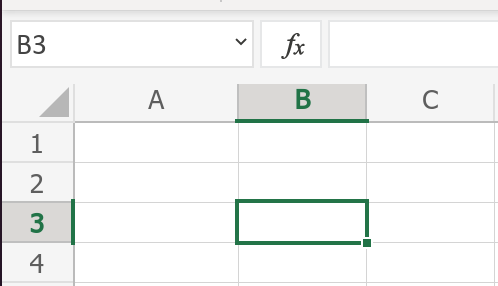
\includegraphics[scale=0.25]{figs/B3}
\end{figure}
I hver celle kan vi skrive inn både tall og tekst. Si at Ole har en jobb med 250\,kr i timelønn, og at han jobber 7 timer i uka. Denne informasjonen kan vi skrive inn i Excel slik:
\begin{figure}[H]
	\centering
	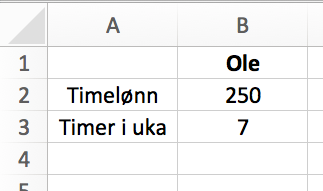
\includegraphics[scale=0.35]{figs/ex2}
\end{figure}
\subsection{Utregninger}
Vi ønsker nå å finne ukelønnen til Ole.
Ukelønnen er gitt ved formelen
\[ \text{ukelønn}={\text{timelønn}\cdot \text{timer i uka}} \]
For å foreta en utregning i regneark, starter man med å skrive {\tt{=}} i cellen. I celle B4 finner vi ukelønnen til Ole ved å skrive {\tt=250$ ^* $7}.
\begin{figure}[H]
	\centering
	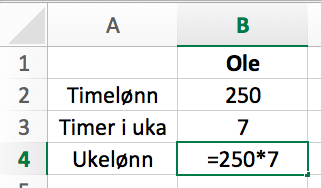
\includegraphics[scale=0.3]{figs/ex3}\qquad
	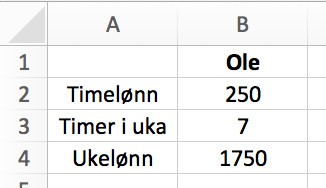
\includegraphics[scale=0.3]{figs/ex4}
\end{figure}
Når vi trykket enter-tasten, er det resultatet, 1750, som vises i cellen. Ønsker vi å se formelen vi har brukt, kan vi dobbeltklikke på cellen, eller se i \textit{inntastingsfeltet} (oppe til høyre i figuren under.)
\begin{figure}[H]
	\centering
	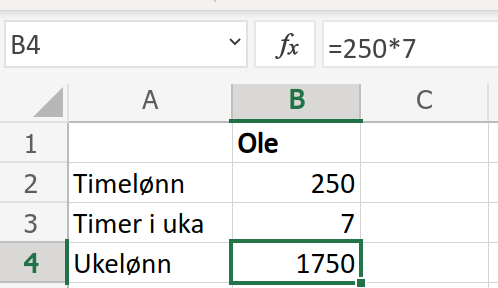
\includegraphics[scale=0.25]{figs/intast}
\end{figure}
\mer Inntastingsfeltet kan også brukes til å taste inn tall og tekst i cellen.

\subsection{Cellereferanser}
Excels kanskje viktigste egenskap er \textit{cellereferanser}. Dette betyr kort sagt at vi bruker celler istedenfor tall når vi skal gjøre utregninger. I forrige seksjon regnet vi lønnen til Ole ved å gange 250 (timelønnen) med 7 (timer i uka). Ved å bruke cellereferanser kunne vi isteden gjort dette:\vsk

Tallet tilhørende timelønnen (250) står i celle B2, mens tallet tilhørende timer (35) står i celle B3. For å gange tallene i disse cellene kan vi skrive {\tt =B2$ ^* $B3}: 

\begin{figure}[H]
	\centering
	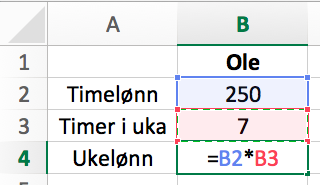
\includegraphics[scale=0.3]{figs/ex5}\qquad
	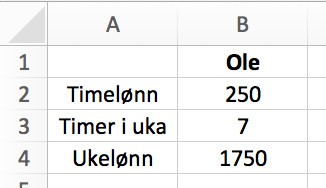
\includegraphics[scale=0.3]{figs/ex4}
\end{figure}
Én av fordelene med å bruke cellereferanser er at det blir mye lettere å rette opp i feil som har blitt gjort. Si f.eks. at det skulle stått 300 istedenfor 250 i B3. Om vi derfor endrer B3, vil resultatet i B4 endre seg deretter:
\begin{figure}[H]
	\centering
	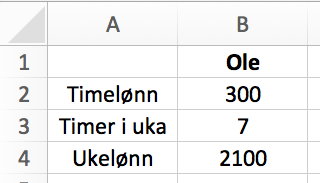
\includegraphics[scale=0.3]{figs/ex6}
\end{figure}
\textsl{Merk:} Du kan også trykke på cellene du ønsker å bruke i formlene dine, slik som vist \net{https://drive.google.com/open?id=1S43og4XFAiYyZeFh7tGClBYXoPSv2i0R}{her}.
\subsection{Kopiering og låsing av celler}
Kopiering av cellene er en metode som hindrer deg i å skrive de samme formlene om og om igjen. Vi ønsker nå å lage at ark som passer til følgende informasjon:
\begin{itemize}
	\item Timelønnen til Ole, Dole og Doffen er henholdsvis 300\,kr, 200\,kr og 500\,kr.
	\item Alle tre jobber 7 dager i uka.
	\item Vi ønsker å regne ut hvor mange timer de jobber til sammen og hvor mye ukelønn de har til sammen.
\end{itemize}

Vi starter med å sette opp dette regnearket:
\begin{figure}[H]
	\centering
	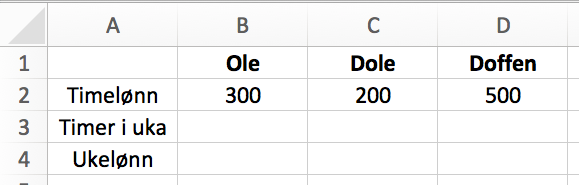
\includegraphics[scale=0.3]{figs/ex7}\qquad
\end{figure}
Her har vi bare fylt inne informasjonen som er \textit{unik} for Ole, Dole og Doffen, nettopp fordi de andre cellene enten inneholder de samme tallene eller den samme regnemåten. For cellene som ikke er unike bør vi bruke kopieringsmulighetene, og dette vises i denne \net{??}{videoen}. Her er en liten beskrivelse av hva som blir gjort:
\begin{enumerate}
	\item Siden alle tre jobber i 7 timer, skriver vi {\tt 7} i celle B4. Etterpå kopierer vi ved å trykke musepekeren helt nede i høyre hjørne av B4 og drar \textsl{bortover} til C2 og D2.
	\item Siden regnemåten av ukelønn er den samme for alle tre, skriver vi den (med cellereferanser) inn i B4, og kopierer den \textsl{bortover} til celle C4 og D4.
	\item Regnemåten for summen av timene og summen av ukelønnene er også den samme, vi skriver den derfor inn i celle E3 og kopierer den \textsl{nedover} til E4.
\end{enumerate}
Resultatet ble dette:
\begin{figure}[H]
	\centering
	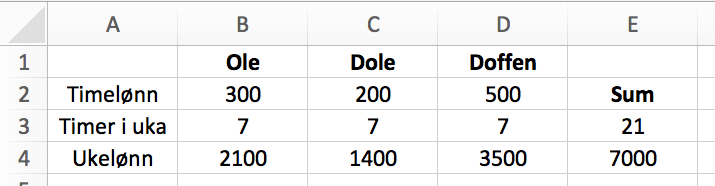
\includegraphics[scale=0.3]{figs/ex8}\\[5pt]
	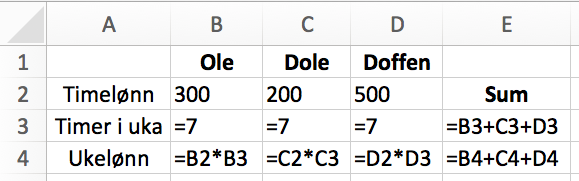
\includegraphics[scale=0.3]{figs/ex15}
\end{figure}
Av det vi har sett i \net{https://drive.google.com/open?id=1FgpfKxFzfrc18sIoy3B1MBfEguvzSzVJ}{videoen} og figurene over kan vi ta med oss to generelle regler:
\begin{enumerate}
	\item Hver gang man kopierer en formel én celle \textsl{bortover}, vil kolonnene i formelen øke med én bokstav i alfabetet. (A blir til B, B blir til C osv.)
		\item Hver gang man kopierer en formel  én celle \textsl{nedover}, vil radene i formelen øke med 1 (1 blir 2 B, 2 blir til 3 osv.).
\end{enumerate}

\textbf{Låsing av celler}\\[2pt]
Når man kopierer celler, er det viktig å se opp for celler man ønsker å bruke i alle kopiene, for disse cellen må \textit{låses}. Si for eksempel at Ole, Dole og Doffen alle jobber 48 arbeidsuker i året. For å finne årslønnen deres må vi altså gange ukeslønnen til hver av dem med 48. \vsk

Igjen merker vi oss at regnemetoden for å finne årslønnen er den samme for alle tre, men hvis vi bruker celle B8 i en formel, og kopierer slik vi har gjort hittil, vil bokstaven B endre seg i formlene. For å unngå dette skriver vi {\tt \$} foran {\tt B} i formelen $ - $ dette gjør at kolonnebokstaven ikke endrer seg, selv om vi kopierer formelen. Dette er vist i denne \net{https://drive.google.com/open?id=1bPz2NYZEB3iWyCMQQYTpgms8LsTepY_G}{videoen}, og resultatet ser vi her:
\begin{figure}[H]
	\centering
	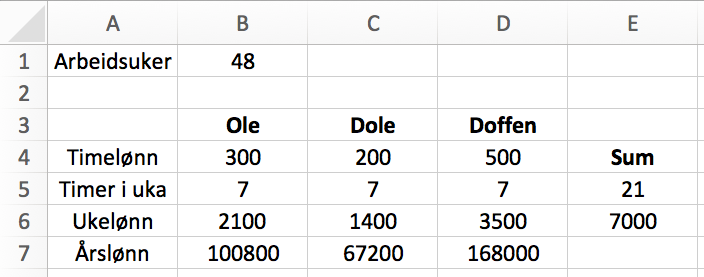
\includegraphics[scale=0.3]{figs/ex12}\\[5pt]
	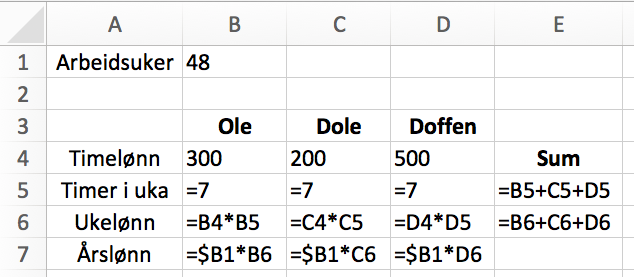
\includegraphics[scale=0.3]{figs/ex13}
\end{figure}
Skal vi låse en celle \textsl{nedover} må vi sette dollaren foran radnummeret, for eksempel {\tt{B\$1}}.
\subsection{Andre nyttige funksjoner}
\st{
\textbf{Videoer}
	\begin{itemize}
	\item \net{https://drive.google.com/file/d/1o7DuDB4yd47kfJWRGXn5Gp3yQbskZiVC/view?usp=sharing}{Sum bort og sum ned}	
	\item \net{https://drive.google.com/file/d/1RoEAzBYq0bkf1T-W_iWfKW4cc4inlRtb/view?usp=sharing}{Justere bredde på kolonne}
	\item \net{https://drive.google.com/file/d/1ZiRWW8CwNgSRvjng6JFxKhFZ5HmWLSXM/view?usp=sharing}{Sette inn rad}
	\item \net{https://drive.google.com/file/d/1iuDPTMvDeA73HCjhXIp9nhdMdWou2qhI/view?usp=sharing}{Formelvisning}
	\item \net{https://drive.google.com/file/d/1EdnLdzkRKL_L7ipeEtNc8wyDlS-f2h9X/view?usp=sharing}{Gjøre om til prosenttall}
	\item \net{https://drive.google.com/file/d/1ueFQnTNYIGEH6lMxXc0o_PWcl7204YVZ/view?usp=sharing}{Endre antall desimaler}
	\item \net{https://drive.google.com/file/d/1HZAlebp51NlwbO5JyxtFPX0TBbvRmvWu/view?usp=sharing}{Sorter i stigende/synkende rekkefølge}
	\item \net{https://drive.google.com/file/d/10era8zDW0oCIcZi8ydT4pFKhxR6b-SUw/view?usp=sharing}{Lage søylediagram}
	\item \net{https://drive.google.com/file/d/1tbXVgy28F4bXqKunZsfYrjiNs-cV6Vk-/view?usp=sharing}{Lage sektordiagram}
	\item \net{https://drive.google.com/file/d/1ueFQnTNYIGEH6lMxXc0o_PWcl7204YVZ/view?usp=sharing}{Lage linjediagram}
\end{itemize}}

\st{
\textbf{Kommandoer} (skrives med {\tt{=}} foran).

\begin{itemize}
	\item {\tt{SUM}(celle1:celle2)} \\
	Summerer alle verdiene fra og med celle1 til og med celle2.
	\item {\tt{AVERAGE}(celle1:celle2)} \\
	Finner gjennomsnittet for alle verdiene fra og med celle1 til og med celle2.
	\item {\tt{MEDIAN}(celle1:celle2)} \\
	Finner medianen for alle verdiene fra og med celle1 til og med celle2.
	\item {\tt{VAR.P}(celle1:celle2)} \\
	Finner variansen for alle verdiene fra og med celle1 til og med celle2.
\end{itemize}	
}

\end{document}